\subsection{Basic concepts}
Let $x_i \in \mathcal X, i=1\ldots,n$ denote a sample of consecutive observations of population activity of $p$ neurons in time bins $i$.  
The activity of each neuron is denoted by the real-valued firing rate, thus  $\mathcal X = \mathbb R^{p\times 1}$.  
For example, in our applicaiton, the firing rate is examplestimated from somatic calcium fluorescence signals with the mean stimulus response subtracted, making it possible for elements of $x_i$ to take on negative values. 

We do not assume that the observations $x_i$ are independently distributed. Rather, the data generating process is assumed to be \emph{ergodic}, \emph{i.e.}\;described by a \emph{true distirbution} $F: \mathcal X \mapsto  \mathbb [0, 1]$ (cumulative) over long periods of time such that the \emph{empirical distribution} $\hat F_n$ from a given sample will convege to $F$ with increasing sample size $n$.

Formally, the emprical distribution is defined as \TODO{this may be unecessary, but I leave it for now.}
\begin{equation}
\hat F_n(x) = \frac 1 n \sum\limits_{i=1}^n \mathbf{1}(x \ge x_i)
\end{equation}
where $\mathbf 1(x \ge x_i)$ is the indicator function which equals 1 when all elements of $x$ are greater than the corresponding elements of $x_i$ and 0 otherwise. \TODO{KJ: Are you using cumulative distributions to avoid binning? DY: Yes. Many theorems such as Glivenko-Catelli Theorem and Skorohod's Representation are proven using  cumulative representation. The empirical distribution is nearly always represented in its cumulative form. Expressing convergence is requires binning or using cumulative; the latter is simpler.}

And, for an ergodic process, $\max\limits_{x\in\mathcal X} \left|\hat F_n(x) - F(x)\right| \to 0$ as $n$ increases.

The true covariance matrix $\Sigma \in \Theta$ is defined as a function of $F$:
\begin{equation}
\Sigma = \int\limits_{z\in\mathcal X} (z - \mu)(z - \mu)^\T \dif F(z)
\quad\mbox{where}\;
\mu = \int\limits_{z\in\mathcal X} z \dif F(z)
\end{equation}
The domain $\Theta$ is the set of all positive-definite $p\times p$ matrices, which is a cone in $\mathbb R^{p\times(p+1)/2}$.

But the usual estimator of the true covariance matrix $\Sigma$ is  the sample covariance matrix:
\begin{equation}
\hat\Sigma_0 =  \frac 1 {n-c} \sum\limits_{i=1}^n (x_i -\hat\mu) (x_i - \hat\mu)^\T
\quad\mbox{where}\;
\hat\mu = \frac 1 n \sum\limits_{i=1}^n x_i
\end{equation}
where $c$ is the sum of temporal correlations \TODO{there must be a better description of this}. For independent observations, $c=1$;  $c>1$ when nearby samples are correlated; the value of $c$ can be estimated from the data.
\TODO{Under the Gaussian loss, $\mathcal L_g$ (\autoref{eq:GaussLoss}) the scaling is irrelevant, so we will not spend any time talking about the scaling.  But it would be important if we used $\mathcal L_e$.} 

$\hat\Sigma_0$ is designed to be unbiased such that $\mathbb E\left[\hat\Sigma_0\right]=\Sigma$.
Here and througout, $\mathbb E[\cdot]$ denotes the expected value under the  unknown true distribution $F$. All variables with a hat (\emph{e.g.}\;$\hat \Sigma_0,\hat \mu$) are functions of the empirical distribution $\hat F_n$, which itself is a random variable.

Nonlinear functions of an unbiased estimate can be biased: $\mathbb E\left[\hat\Sigma_0\right]=\Sigma \centernot\implies  E\left[\varphi(\hat\Sigma_0)\right]=\varphi(\Sigma)$.  For example, if $u_{\max}(S)$ is the largest eigevalue of square matrix $S$, then $\mathbb E\left[u_{\max}(\hat\Sigma_0)\right] > u_{\max}(\Sigma)$. Some covariance matrix estimators are designed to correct for the eigenspectrum bias at the cost of adding bias to covariance coefficients \citep{Ledoit:2004}.




\subsection{Loss functions and risk}
The optimization of a covariance matrix estimate $\hat\Sigma$ is performed with respect to a \emph{loss function} $\mathcal L(\hat\Sigma,\Sigma)$, which expresses the discrepancy between $\hat\Sigma$ and $\Sigma$ and attains its minimum when $\hat\Sigma=\Sigma$.  
Then \emph{excess loss}  
\begin{equation}
\ell(\hat\Sigma,\Sigma) = \mathcal L(\hat\Sigma,\Sigma)-\mathcal L(\Sigma,\Sigma)
\end{equation}
assumes zero at its minimum.

A particularly useful loss function is the mean squared error (MSE), which is proportional to the square of the Frobenius  norm $\|\cdot\|_F$ of the difference between the matrices: 
\begin{equation}\label{eq:MSE}
\mathcal L_e(\hat\Sigma,\Sigma) =\frac 1 p \|\hat\Sigma-\Sigma\|_F^2 = \frac 1 p \Tr\left((\hat \Sigma-\Sigma)(\hat\Sigma-\Sigma)^\T\right)
\end{equation}
The MSE is its own excess loss: $\ell_e(\hat\Sigma,\Sigma) \equiv \mathcal L_e(\hat\Sigma,\Sigma)$.

The Gaussian loss function $\mathcal L_g$  arises from the theory of multivariate normal distributions. When observations are identically and independently distributed according to a multivariate normal distribution with zero means, the log likelihood of the covariance matrix $\Sigma$ with $\hat\Sigma = \frac 1 n \sum\limits_{i=1}^n x_i x_i^\T$ is  
\begin{equation}
L\left(\Sigma \mid \hat\Sigma\right) = -\frac n 2 \ln(2\pi) - \frac n 2 \ln \det \Sigma - \frac n 2 \Tr(\Sigma^{-1} \hat \Sigma)
\end{equation}
Then $\mathcal L_g$ is constructed by rescaling $L\left(\Sigma \mid \hat\Sigma\right)$ and dropping the constant term:
\begin{equation}\label{eq:GaussLoss}
\mathcal L_g(\hat\Sigma,\Sigma) 
=  -\frac 2 {pn} L\left(\Sigma \mid \hat\Sigma \right) - \frac 1 p \ln(2\pi) 
\equiv  \frac 1 p\left(\ln \det \hat \Sigma + \Tr(\hat \Sigma^{-1}) \right) 
\end{equation}
The corresponding excess loss 
\begin{equation}
\ell_g(\hat\Sigma,\Sigma) = \mathcal L_g(\hat\Sigma,\Sigma) - \mathcal L_g(\Sigma,\Sigma)  
= \frac 1 p \left(-\ln \det (\hat \Sigma^{-1} \Sigma) + \Tr(\hat \Sigma^{-1}\Sigma)\right) - 1
\end{equation}
is known as \emph{entropy loss} \citep{James:1961}.

Despite the fact that entropy loss is derived from normal theory, the choice of a loss function is not equivalent to assuming a specific form of $F$. The loss function measures the discrepancy between distribution parameters rather than the distance between the distributions themselves. \TODO{explain Bregman divergence?} 

The expected value of excess loss is the \emph{estimator risk}:
\begin{equation}\label{eq:risk}
r = \mathbb E\left[\ell(\hat\Sigma,\Sigma)\right]
\end{equation}
The estimator risk is the primary quality criterion for covariance estimation. Estimator $\hat\Sigma_a$ is considered more \emph{efficient} than estimator $\hat\Sigma_b$ if $\hat\Sigma_a$ has lower risk for the given sample than $\hat\Sigma_b$.   \TODO{explain that the risk depends not only on $\hat\Sigma$ but also on the distribution of $\Sigma$ in the specific domain.}

\subsection{Cross validation}
In practice, the true covariance matrix $\Sigma$ is not accessible and the estimator risk $r$ must be estimated from data. This requires a separate \emph{validation} empirical distribution $\hat F_m^\prime$ of $m$ observations sampled from $F$ independently of the \emph{training} distribution $\hat F_n$. 
Then let  $\hat \Sigma_0^\prime$ be the sample covariance obtained from $\hat F_m^\prime$. 

Then the \emph{empirical loss} of $\hat\Sigma$ is $\mathcal L(\hat\Sigma,\hat\Sigma_0)$ and its expectation is the \emph{empirical risk}  
\begin{equation}
\hat r = \mathbb E\left[\mathcal L(\hat\Sigma,\hat\Sigma_0^\prime)\right]
\end{equation}

 The two loss functions $\mathcal L_e(\hat\Sigma,\Sigma)$ and $\mathcal L_g(\hat\Sigma,\Sigma)$ are particularly suitable for risk estimation thanks to their linearity with respect to $\Sigma$ in the sense that 
\begin{equation}
\mathcal L\left(\hat\Sigma,\alpha S_1 + (1-\alpha)S_2\right) 
\equiv 
\alpha\mathcal L(\hat \Sigma,S_1) + (1-\alpha)\mathcal L(\hat \Sigma,S_2)
\end{equation}
which allows bringing the expectation inside the empirical loss function:
\begin{equation}
\hat r = 
\mathbb E\left[ \mathcal L(\hat\Sigma, \hat\Sigma_0^\prime) \right] 
=
\mathbb E\left[ \mathcal L\left(\hat\Sigma, \mathbb E\left[\hat\Sigma_0^\prime\right]\right) \right] 
=
\mathbb E\left[ \mathcal L(\hat\Sigma, \Sigma) \right] 
= 
r + \mathcal L(\Sigma,\Sigma)
\end{equation}
This means, that the empirical loss $\mathcal L(\hat\Sigma,\hat\Sigma_0^\prime)$ is an unbiased estimate of the estimator risk $r$ (up to a constant offset): minimization of the empirical loss implies minimization of the true estimator risk. 

Recording a separate independent validation sample is usually not sensible.  Instead, the recorded data are split into a training sample and validation sample. In $K$-fold \emph{cross-validation} the data are split into $K$ roughly equal-sized subsets. Each subset then successively serve as the testing sample while the remainder of the data serves as the training sample.  This procedure produces $K$ estimates of the  risk, which are then averaged together to produce a better averaged estimate.


\subsection{Bias/variance decomposition}
The estimator risk (\autoref{eq:risk}) can be decomposed into \emph{approximation error} or \emph{bias}   
\begin{equation}
b^2 = \ell \left( \mathbb E[\hat \Sigma],\Sigma\right)
\end{equation}
and \emph{estimation error} or \emph{variance}
\begin{equation}
\varepsilon^2 = \mathbb E \left[ \ell\left(\hat \Sigma, 
\mathbb E[\hat \Sigma]\right) \right]
\end{equation}

Under the MSE loss function $\mathcal L_e$ (\autoref{eq:MSE}), the decomposition is the simple sum $r = b^2 + \varepsilon^2$. 
Under other loss functions, $r$ is an increasing function of both $b^2$ and $\varepsilon^2$ although not generally a simple sum.  
\TODO{As far as I know, the terms `bias' and `variance' are only applicable under a quadratic loss function  like $\mathcal L_e$.  Under other loss functions, we may need to use approximation/estimation error.} 

The sample covariance matrix $\hat\Sigma_0$ has zero bias but high variance. Other estimators may be biased but have lower estimation error and potentially lower risk.


\subsection{Regularization}

\emph{Regularization} is the deliberate biasing (`shrinkage') of the unbiased estimate toward a less variable low-dimensional \emph{target estimate} $\hat T$ in order to minimize the estimator risk by striking a favorable balance between bias and variance.
A regularized covariance matrix estimator must solve two problems: (a) choose and fit the target covariate estimate $\hat T$ and (b) mix $\hat\Sigma_0$ with $\hat T$ by the optimal amount. 
Regularized covariance matrix estimates can be generally expressed as 
\begin{equation}
\hat\Sigma_{d,\lambda} = mix(\Sigma_0,\hat T_{\hat d},\hat\lambda) 
\end{equation}
where $\hat d$ indicates the choice of the target estimate from the family of target estimates $\hat T_d$. $mix(\cdot,\cdot,\hat\lambda)$ is the mixing function of $\hat\Sigma_0$ and $\hat T_{\hat d}$ in proportion controlled by $\hat \lambda$. Both $\hat d$ and $\hat \lambda$ must be calculated from the training sample. 

A number of regularization schemes have been developed, which differ by their target estimates and mixing functions.    Curiously, \emph{some} improvement can be produced with an arbitrary target estimate as long as its variance is lower than that of $\hat\Sigma_0$.  The perplexing phenomenon that estimates can be improved by a bias toward an arbitrary less variable target is known as \emph{Stein's paradox} \citep{Efron:1977}.   \TODO{This point can be untuitive.  For example, \cite{Varoquaux:2012} misrepresents the effect of regularization by stating that regularization removes the upward bias of correlations in the sample covariance matrix. In reality, regularization should start with an unbiased estimator and bias it toward a low-variance target so that the estimation risk is reduced.} However, if a family of target estimates can capture the underlying regularities in the covariance structure of a specific system with a small number of parameters, biasing the estimate toward these targets ought to produce a greater reduction in estimator risk. 

In this study, we evaluate four regularized estimators whose target estimates correspond to the graphical models in Figure \ref{fig:02}: diagonal (A), multifactor (B), sparse partial correlations (C), and sparse  partial correlations with latent units (D).  The following describe each regularization scheme separately.

\begin{figure}[htp]
\centering
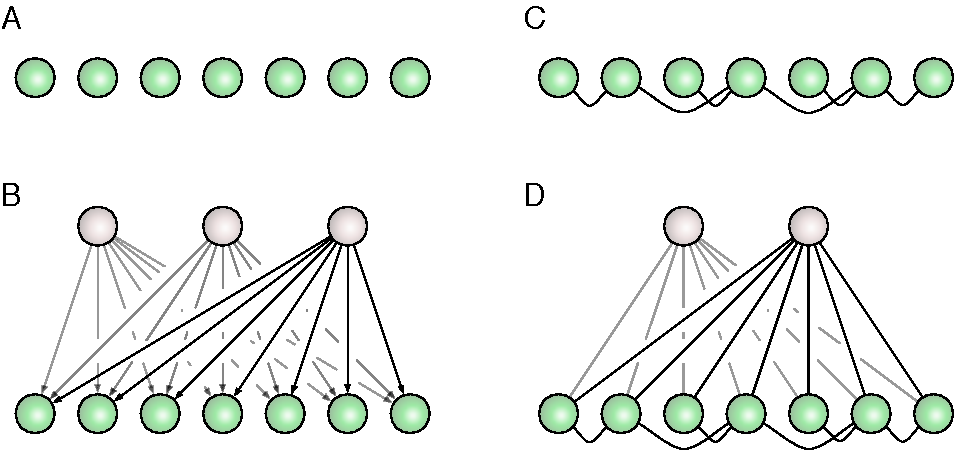
\includegraphics[width=0.5\textwidth]{figures/Figure2.pdf}
\caption{
Graphical models corresponding to the low-dimensional targets of the four regularization schemes used in the paper.
\textbf{A}: A diagonal matrix corresponds to a Gaussian graphical model with no dependencies. 
\textbf{B}: In factor analysis, observed nodes are assumed to be influenced by several latent units (``factors") but are otherwise independent. 
\textbf{C}: In the Gaussian graphical model (also known as the Gaussian Markov Field), correlations arise from sparse pairwise linear interactions between visible units. 
\textbf{D}: In the Gaussian graphical model with latent units, correlations arise  between pairs of nodes 
}\label{fig:02}
\end{figure}

\subsection{Estimator A: Shrinkage toward diagonal}
The most popular covariance regularization schemes use diagonal target estimates and linear shrinkage toward the target.  For example, the target could be the identity matrix:  
\begin{equation}
\hat T = \hat v I
\end{equation}
where $\hat v = \frac 1 p \sum\limits_{i=1}^p(\hat\Sigma_0)_{ii}$ is the mean sample variance. 

Alternatively, the target could contain the sample variances:
\begin{equation}
\hat T= \hat\Sigma_0 \circ I 
\end{equation}
where $\circ$ is the entrywise matrix product.

Finally, the target could be a linear mixture of the common variance and independent variance targets
\begin{equation}
\hat T_{\hat\eta} = (1-\hat\eta)(\hat\Sigma_0 \circ I) + \hat\eta\hat v I
\end{equation}

The regularized estimator is the linear mixture of $\hat\Sigma_0$ and $\hat T_{\hat\eta}$:
\begin{equation}
\hat\Sigma_{\hat\eta,\hat\lambda} = (1-\hat\lambda)\hat\Sigma_0 + \hat\lambda \hat T_{\hat\eta} 
\end{equation}

The hyperparameters $\hat\eta$ and $\hat\lambda$ must be estimated from the data.  Under the MSE loss function $\mathcal L_e$ (\autoref{eq:MSE}), the optimal values of $\hat\eta$ and $\hat\lambda$ can be estimated analytically \citep{Ledoit:2004,Schafer:2005,Schaefer:2010}. However, these estimates are no longer optimal under the Guassian loss $\mathcal L_g$. \TODO{I have tested this and there was a substantial difference in both synthetic and empirical data}  When an analytical solution for optimal hyperparameters is not available, the optimal values can be found by cross validation, entirely within the the training sample. \TODO{explain nested cross-validation in more detail?}

\TODO{Describe how the empirical loss is convex in the hyperparameters in this case}

\subsection{Estimator B: Shrinkage toward a factor model}
In estimator B, the target is a factor model, composed as the sum of a low-rank component $\hat L_{\hat d}\hat L_{\hat d}^\T$ and a diagonal matrix $\hat \Psi$:
\begin{equation}
\hat T_{\hat d} = \hat L_{\hat d} \hat L_{\hat d}^\T + \hat\Psi
\end{equation}
Here $\hat L_{\hat d}$ is an $p\times\hat d$ matrix and $\hat\Psi$ is diagonal.  

If $F$ were assume to be multivariate normal \TODO{or other distributions that are defined by linear dependencies}, the factor model is corresponds to the graphical model (\autoref{fig:02}B) where the activity of all neurons are dependent only $\hat d$ latent units. This suggest a mechanistic interpretation in which the interactions between neurons are insignificant compared to the influence of inputs outside the recorded circuit.

Just as in Estimator A, Estimator B is allowed to only partially commit to the low-dimensional target: the overall estimate is the linear mixture of the sample covariance and the target
%\begin{equation}
%\hat\Sigma_{\hat d,\hat\lambda} = (1-\hat\lambda)\hat\Sigma_0 + \hat  
%\end{equation}

\TODO{Check \citep{Fan:2011,Fan:2006}}

\subsection{Estimator C: Sparse partial correlations}
\citep{Meinshausen:2006,Friedman:2008}

\subsection{Estimator D: Sparse partial correlations with latent units}
\citep{Ma:2013} 


